% !TeX root = ./ms.tex
\documentclass[modern]{aastex62}

% Load the corTeX style definitions
% !TeX root = ./ms.tex
% All the packages
\usepackage{url}
\usepackage{amsmath}
\usepackage{mathtools}
\usepackage{amssymb}
\usepackage{natbib}
\usepackage{graphicx}
\usepackage{calc}
\usepackage{etoolbox}
\usepackage{xspace}
\usepackage[T1]{fontenc} % https://tex.stackexchange.com/a/166791
\usepackage{textcomp}
\usepackage{ifxetex}
\ifxetex
\usepackage{fontspec}
\defaultfontfeatures{Extension = .otf}
\fi
\usepackage{fontawesome}
\usepackage{listings}
\usepackage{nicefrac}
\usepackage[bb=boondox]{mathalfa}
\usepackage{booktabs}
\usepackage{longtable}

% Shorthand for this paper
\newcommand{\starry}{\textsf{starry}\xspace}
\newcommand{\Python}{\textsf{Python}\xspace}
\newcommand{\cpp}{\textsf{C}++\xspace}
\newcommand{\bvec}[1]{{\ensuremath{\mathbf{#1}}}}
\newcommand{\xxx}[1]{{\color{red}#1}}
\DeclarePairedDelimiter\floor{\lfloor}{\rfloor}
\DeclarePairedDelimiter\ceil{\lceil}{\rceil}
\newcommand{\imag}{{\ensuremath{\mathbb{i}}}}
\newcommand{\quadquad}{\quad\quad\quad\quad}

\newcommand{\R}{\bvec{R}}
\newcommand{\AOne}{\bvec{A_1}}
\newcommand{\alm}{\bvec{a}}
\newcommand{\x}{\bvec{x}}
\newcommand{\D}{D}
\newcommand{\Doppler}{\bvec{D}}
\newcommand{\Surf}{\mathcal{S}}
\newcommand{\Curve}{\mathcal{C}}
\newcommand{\Dargs}{\bvec{d}}
\newcommand{\lmax}{\ensuremath{l_\mathrm{max}}}
\newcommand{\spot}{\texttt{SPOT}\xspace}
\newcommand{\vogtstar}{\texttt{VOGTSTAR}\xspace}
\newcommand{\kT}{\boldsymbol{\kappa}^\top}
\newcommand{\rhoT}{\boldsymbol{\rho}^\top}
\newcommand{\ylmbasis}{\boldsymbol{\psi}^\top}
\newcommand{\pbasis}{\boldsymbol{\phi}^\top}
\newcommand{\pbasisn}{\ensuremath{\phi_n}}
\newcommand{\azero}{\ensuremath{\bvec{a_0}}}

% References to text content
\newcommand{\documentname}{\textsl{article}}
\newcommand{\figureref}[1]{\ref{fig:#1}}
\newcommand{\Figure}[1]{Figure~\figureref{#1}}
\newcommand{\figurelabel}[1]{\label{fig:#1}}
\renewcommand{\eqref}[1]{\ref{eq:#1}}
\newcommand{\Eq}[1]{Equation~(\eqref{#1})}
\newcommand{\eq}[1]{\Eq{#1}}
\newcommand{\eqalt}[1]{Equation~\eqref{#1}}

% Add code, proof, and animation hyperlinks
\definecolor{linkcolor}{rgb}{0.1216,0.4667,0.7059}
\newcommand{\codeicon}{{\color{linkcolor}\faFileCodeO}}
\newcommand{\prooficon}{{\color{linkcolor}\faPencilSquareO}}
\newcommand{\codelink}[1]{\href{https://github.com/user/repo/blob/cfda45841cf4235e82cf705ab27251bd783bdf8c/tex/figures/#1.py}{\codeicon}\,\,}
\newcommand{\animlink}[1]{\href{https://github.com/user/repo/blob/cfda45841cf4235e82cf705ab27251bd783bdf8c/tex/figures/#1.gif}{\animicon}\,\,}
\newcommand{\prooflink}[1]{\href{https://github.com/user/repo/blob/cfda45841cf4235e82cf705ab27251bd783bdf8c/tex/proofs/#1.ipynb}{\raisebox{-0.1em}{\prooficon}}}
\newcommand{\cilink}[1]{\href{https://dev.azure.com/user/repo/_build}{#1}}


% Define a proof environment for open source equation proofs
\newtagform{eqtag}[]{(}{)}
\newcommand{\currentlabel}{None}
\newenvironment{proof}[1]{%
\ifstrempty{#1}{%
\renewtagform{eqtag}[]{\raisebox{-0.1em}{{\color{red}\faPencilSquareO}}\,(}{)}%
}{%
\renewtagform{eqtag}[]{\prooflink{#1}\,(}{)}%
}%
\usetagform{eqtag}%
\renewcommand{\currentlabel}{#1}
\align%
}{%
\endalign%
\renewtagform{eqtag}[]{(}{)}%
\usetagform{eqtag}%
\message{<<<\currentlabel: \theequation>>>}%
}

% Display the runtime on Azure
\usepackage[skins]{tcolorbox}
\newtcbox{\figtimebox}{enhanced,nobeforeafter,tcbox raise=-0.8mm,boxrule=0.6pt,
  top=0.5mm,bottom=0mm,right=0mm,left=6mm,arc=1pt,boxsep=2pt,
  before upper={\vphantom{dlg}},colframe=linkcolor,coltext=linkcolor,
  fontupper=\sffamily\bfseries\tiny,colback=white,overlay={\begin{tcbclipinterior}
  \fill[linkcolor] (frame.south west)
  rectangle node[text=white,font=\sffamily\bfseries\tiny,rotate=0]{CPU} 
  ([xshift=6mm]frame.north west);\end{tcbclipinterior}}}
\robustify{\figtimebox}
\pdfstringdefDisableCommands{%
  \def\figtimebox#1{'#1'}%
}
\newcommand{\figtime}[1]{\IfFileExists{figures/#1.py.time}%
{%
\cilink{\figtimebox{\input{figures/#1.py.time}\unskip s}}
}{}}

% Define the `oscaption` command for open source figure captions
\newcommand{\oscaption}[2]{\caption{#2 \codelink{#1} \figtime{#1}}}

% Code examples
\definecolor{codegreen}{rgb}{0,0.6,0}
\definecolor{codegray}{rgb}{0.5,0.5,0.5}
\definecolor{codepurple}{rgb}{0.58,0,0.82}
\definecolor{backcolour}{rgb}{0.95,0.95,0.95}
\lstdefinestyle{mystyle}{
    backgroundcolor=\color{backcolour},
    commentstyle=\color{codegreen},
    keywordstyle=\color{magenta},
    numberstyle=\tiny\color{codegray},
    stringstyle=\color{codepurple},
    basicstyle=\small\ttfamily,
    breakatwhitespace=false,
    breaklines=true,
    captionpos=b,
    keepspaces=true,
    numbers=left,
    numbersep=5pt,
    showspaces=false,
    showstringspaces=false,
    showtabs=false,
    tabsize=2,
    aboveskip=1em,
    belowskip=1em,
    keywords=[2]{map},
    keywordstyle=[2]{\color{black!80!black}},
    upquote=true
}
\lstset{style=mystyle}

% Typography obsessions
\setlength{\parindent}{3.0ex}
\renewcommand\quad{\hskip\fontdimen3\font}

% https://tex.stackexchange.com/a/184474
\usepackage{stackengine,scalerel}
\def\lnlam{\ThisStyle{\ensurestackMath{\stackon[-2.4\LMpt]{%
  \SavedStyle\lambda}{\kern-.5pt\kern\LMpt\rule{1\LMex}{.25pt+.15\LMpt}}}}}

% Bibliography stuff
\bibliographystyle{aasjournal}

% Begin!
\begin{document}

% Title
%\title{Inferring a time dependent map of Io's surface from occultations and phase curves.}
\title{Time-variable surface mapping of exoplanets: an application to Io}

% Author list
\author{Fran Bartoli\'c}
\email{fbartolic@flatironinstitute.org}
\affil{Center~for~Computational~Astrophysics, Flatiron~Institute, New~York, NY}
\affil{Centre for Exoplanet Science, SUPA, School of Physics and Astronomy, University of St. Andrews, St. Andrews, UK}
\author{Rodrigo Luger}
\author{Daniel Foreman-Mackey}
\affil{Center~for~Computational~Astrophysics, Flatiron~Institute, New~York, NY}
%

\begin{abstract} 
Jupiter's moon Io is the most volcanically active body in the Solar System with hundreds of active volcanoes varying in intensity on different timescales. 
Existing photometric observations in the near infrared taken during occultations by Jupiter and Galilean moons encode a wealth of information about its surface. 
As such, Io is an ideal testbed for models of time-variable exoplanet surfaces. 
We build a single probabilistic model of Io's surface using Nonnegative Matrix Factorization to infer one map per light curve.
The model is built on top of the code Starry \href{https://rodluger.github.io/starry/}{\color{linkcolor}\faGithub} which can compute occultation light curves and phase curves in both emitted and reflected light. It also enables efficient inference with gradient based samplers. 
We use the inferred map to study the time variability of prominent volcanoes over a timescale of decades.
While we mostly focus on Io, the lessons we learn are directly applicable to mapping exoplanets. 
We discuss this application towards the end of the paper.\href{https://github.com/fbartolic/volcano}{\color{linkcolor}\faGithub}

\end{abstract}

%
\section{Introduction}
The surface of Jupiter's moon Io is littered with hundreds of volcanoes appearing as bright spots in the near infrared and varying in intensity on timescales of days to decades.
The volcanic activity is driven by tidal interactions with Jupiter and sustained by the Laplace resonance with Europa and Ganymede \citep{peale_melting_1979}.
Io is a perfect analogue of an extremely volcanically active exoplanet.
Such rocky exoplanets, often dubbed \emph{super-Ios} or \emph{lava worlds}, have gathered a lot of interest in recent years because the photometric and spectral signatures of volcanic activity on such worlds will likely be detectable in the near future \citep{kaltenegger_detecting_2010,henning_highly_2018,oza_sodium_2019}.
Studying volcanism on both Io and exoplanets is scientifically valuable because it provides a window into the properties of early Earth and it informs theories of planet formation.

Existing exoplanet detections with potential volcanism include CoRoT-7b \citep{barnes_corot-7b_2010}, the first discovered rocky exoplanet with likely significant tidal heating; 55 Cancri e, whose longitudinal offset in peak surface emission has been attributed to, among other things, lava flows on the surface \citep{demory_variability_2016,demory_map_2016,hammond_linking_2017}; several planets in the TRAPPIST-1 system in a Laplace-like resonance with likely volcanic activity \citep{kislyakova_magma_2017,dobos_tidal_2019}; and many others.
Not all exoplanets will have Io-like volcanism, some will have magma oceans due to their proximity to the star or volcanism caused by nuclear decay similar to early Earth volcanism.

Io has been observed extensively using both space and ground observatories.
High resolution images of Io's surface were taken by space missions such as Voyager \citep{smith_jupiter_1979}, Galileo \citep{belton_galileos_1996} and Juno \citep{mura_infrared_2020}.
It has also been resolved from the ground in the near infrared using disk resolved imaging
\citep{howell_infrared_1985,simonelli_disk-resolved_1986,spencer_discovery_1990} and adaptive optics observations \citep{marchis_adaptive_2000,marchis_keck_2005,de_kleer_spatial_2016}.
Most importantly for this work, Io has been sporadically observed for decades using high cadence near infrared photometry taken during occultations by Jupiter starting with \cite{spencer_discovery_1990}.
Occultations by Jupiter occur twice every orbit lasting ~1.7 days and mutual occultations with Europa, Ganymede or Callisto happen every ~6 years when Earth pasess through the orbital plane of Galilean satellites.
The majority of occultations by Jupiter are observed when Io is in Jupiter's shadow ("in eclipse") while mutual occultations are almost always observed in sunlight because mutual occultations while Io is in eclipse are extraordinarily rare.
Only the brightest volcanoes are visible over the reflected light background when Io is illuminated by the Sun\citep{veeder_ios_1994,de_kleer_spatial_2016}.

Both kinds of occultations have been used to study volcanic activity on the surface.
\cite{spencer_io_1994} observed several occultations of Io by Europa and detected a major brightening of the most powerful of Io's volcanoes, Loki, relative to previous Voyager observations.
\cite{rathbun_loki_2002, rathbun_loki_2006,rathbun_ground-based_2010} used observations from NASA's IRTF telescope to study the long term variability of different volcanic spots finding evidence of periodicity in Loki's eruptions and established the transient nature of the volcanoes (only Loki is persistently active).
By studying an occultation of Io by Europa, \cite{de_kleer_multi-phase_2017} mapped the Loki region to a precision of about 2 kilometers.
In addition to observations of occultations in near infrared, several groups have been observing mutual occultations in the optical \citep[][and references therein]{arlot_mutual_1974,saquet_phemu15_2018,morgado_astrometry_2016} with the purpose of inferring the optical albedo of Io and improving ephemeris precision for Galilean satellites.

None of the studies of occultations in the infrared attempted to infer a two-dimensional map of Io's surface. 
The light curves are usually fit independently with the goal of inferring one-dimensional longitudinal variations in brightness on its surface.
Strong priors on the locations of individual volcanoes are assumed based on maps from space mission observations.
In this work, we build a fully probabilistic model in order to infer a time-dependent two-dimensional \emph{map} of Io's volcanic surface from archival IRTF observations in the near infra red.
The model is built on top of the recently developed code Starry \citep[][Luger et al. 2020 in prep]{luger_starry_2019} which 
enables fast analytic computation of occultation light curves and phase curves for objects whose surface features are represented in terms of spherical harmonics.
Starry can compute phase curves and occultations in both emitted light (for modeling the isotropic volcanic emission from Io's surface) and reflected light (for mapping albedo variations).
Instead of fitting one map per occultation light curve, we reduce the dimensionality of the problem using matrix factorization, assuming a fixed map for a given light curve which is a linear combination of $K$ basis maps.
We use priors on the map features which ensure the maps are physical and prevent overfitting of the data.
The model is interpretable, each of the basis maps roughly corresponds to a single spot on the surface, and the coefficients multiplying the basis maps encode information on the time variability.

Our goals for this paper are to both improve on past studies of Io using occultation light curves and to construct a flexible model directly applicable to future efforts on inferring time-dependent maps of variable features on exoplanet surfaces such as volcanoes, magma oceans or clouds.
The fact that we have lots of prior information on what the surface of Io should look like enables us to test our model in a realistic setting, testing sensitivity to chosen priors, data quality, the orbital parameters and different kinds of surface features. 

The paper is organized as follows.
In \S\ref{sec:data} we describe the IRTF light curves of occultations by Jupiter which we use to infer maps. 
In \S\ref{sec:model} we discuss the generative model for the data for the case of a static map, and a dynamic map modeled using a matrix factorization approach and we write down the relevant likelihood functions.
In \S\ref{sec:inverse_problem} we focus on the question of how to do Bayesian inference given the forward model specifications defined in \S\ref{sec:model}. 
We discuss and test different priors on map features, the information content of light curves and fitting the models using variational inference (VI) methods and Hamiltonian Monte Carlo (HMC).
We present results on simulated data.
\S\ref{sec:results} shows the results on real data.
In particular, the inferred dynamic map, the  different component maps and accompanying coefficients, the uncertainties of the maps, sensitivity to different choices of priors, comparison of inferred locations and intensities of spots to known values from the literature.
Finally, in \S\ref{sec:exoplanets} we discuss applications of the model to future exoplanet obervations and test the model predictions on simulated JWST observations of a volcanic Super-Earth.

\section{Data}
\label{sec:data}
\section{Model}
\label{sec:model}
% Discuss starry, pixels vs. schmixels vs. harmonics, forward model for static map, NMF model for dynamic map
\subsection{Orbital parameters}
\label{ssec:orbital_parameters}
% Talk about JPL horizons, uncertainties on parameters, geometry of occultations etc.

\section{The inverse problem}
\label{sec:inverse_problem}
% bulk of the results in the paper
\subsection{The information content of a light curve}
% information in different kinds of occultations/phase curves, reflected light vs. emitted light, posterior shrinkage etc.

\label{ssec:information_content}
\begin{figure}[h!]
    \begin{centering}
    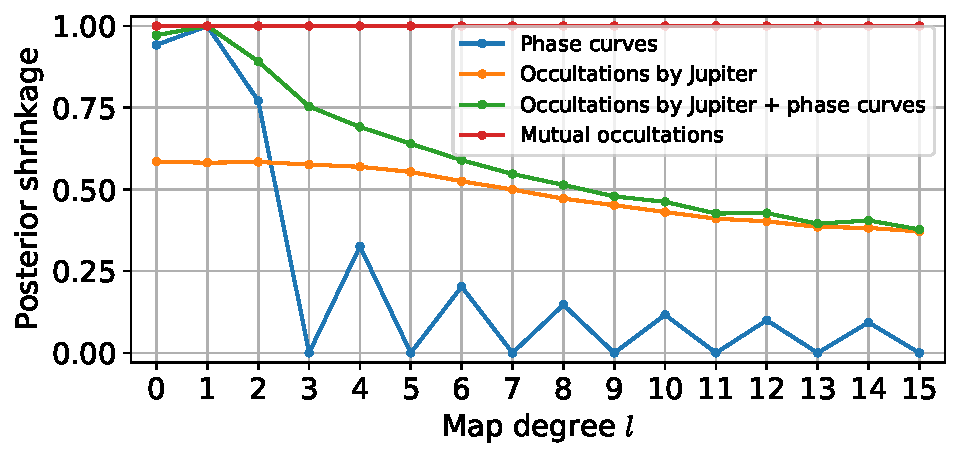
\includegraphics[width=0.5\linewidth]{figures/information_content.pdf}
    \oscaption{InformationContent}{%
        This is a plot of a pretty function. And at the end of this
        caption is a symbol with a link to the \emph{exact} script
        that generated it, hosted on \textsf{GitHub}.
        \label{fig:information_content}
    }
    \end{centering}
\end{figure}

\subsection{Fitting a static map}
\label{ssec:static_map}
% Priors for static maps, sparsity, positivity, plot of map inference with simulated data and different kinds of priors. Inference with MAP, VI, HMC.

\subsection{Fitting a dynamic map}
\label{ssec:dynamic_map}
% Priors for NMF. Optimization vs. bayesian approach to NMF. Results on simulated data. Comparison of results to matrix factorization without the positivity constraint and clever priors.

\section{Results}
\label{sec:results}

\subsection{Individual events}
\label{ssec:individual}
% Fits of individual events. In particular, those light curves that were analyzed in previous papers. 

\subsection{The time-variable map}
\label{ssec:time_variable_map}
% 

\subsection{Variability of known hotspots}
\label{ssec:variability_hotspots}
% Plot inferred intensities of known hotspots as function of time, reference previous work.

\section{Mapping volcanic exoplanets}
\label{sec:exoplanets}
% Application to exoplanets. Fitting mock JWST observations.

% Bibliography
\bibliography{bib}
\end{document}
